%%%%%%%%%%%%%%%%%%%%%%%%%%%%%%%%%%%%%%%%%
% Beamer Presentation
% LaTeX Template
% Version 1.0 (10/11/12)
%
% This template has been downloaded from:
% http://www.LaTeXTemplates.com
%
% License:
% CC BY-NC-SA 3.0 (http://creativecommons.org/licenses/by-nc-sa/3.0/)
%
%%%%%%%%%%%%%%%%%%%%%%%%%%%%%%%%%%%%%%%%%

%----------------------------------------------------------------------------------------
%	PACKAGES AND THEMES
%----------------------------------------------------------------------------------------

\documentclass{beamer}

\mode<presentation> {

% The Beamer class comes with a number of default slide themes
% which change the colors and layouts of slides. Below this is a list
% of all the themes, uncomment each in turn to see what they look like.

%\usetheme{default}
% \usetheme{AnnArbor}
%\usetheme{Antibes}
%\usetheme{Bergen}
% \usetheme{Berkeley}
% \usetheme{Berlin}
%\usetheme{Boadilla}
%\usetheme{CambridgeUS}
%\usetheme{Copenhagen}
%\usetheme{Darmstadt}
%\usetheme{Dresden}
% \usetheme{Frankfurt}
%\usetheme{Goettingen}
%\usetheme{Hannover}
%\usetheme{Ilmenau}
%\usetheme{JuanLesPins}
%\usetheme{Luebeck}
% \usetheme{Madrid}
%\usetheme{Malmoe}
%\usetheme{Marburg}
%\usetheme{Montpellier}
%\usetheme{PaloAlto}
%\usetheme{Pittsburgh}
%\usetheme{Rochester}
\usetheme{Singapore}
%\usetheme{Szeged}
% \usetheme{Warsaw}

% As well as themes, the Beamer class has a number of color themes
% for any slide theme. Uncomment each of these in turn to see how it
% changes the colors of your current slide theme.

%\usecolortheme{albatross}
%\usecolortheme{beaver}
%\usecolortheme{beetle}
%\usecolortheme{crane}
% \usecolortheme{dolphin}
%\usecolortheme{dove}
%\usecolortheme{fly}
% \usecolortheme{lily}
% \usecolortheme{orchid}
%\usecolortheme{rose}
%\usecolortheme{seagull}
%\usecolortheme{seahorse}
%\usecolortheme{whale}
%\usecolortheme{wolverine}

%\setbeamertemplate{footline} % To remove the footer line in all slides uncomment this line
%\setbeamertemplate{footline}[page number] % To replace the footer line in all slides with a simple slide count uncomment this line

%\setbeamertemplate{navigation symbols}{} % To remove the navigation symbols from the bottom of all slides uncomment this line
}
\usepackage{caption}
\usepackage{graphicx} % Allows including images
\usepackage{booktabs} % Allows the use of \toprule, \midrule and \bottomrule in tables

%----------------------------------------------------------------------------------------
%	TITLE PAGE
%----------------------------------------------------------------------------------------

\title[Short title]{VE311 FINAL RC - Single Stage Amplifier} % The short title appears at the bottom of every slide, the full title is only on the title page

\author{Runxi Wang} % Your name
\institute[UN-SJTU JI] % Your institution as it will appear on the bottom of every slide, may be shorthand to save space
{
UM-SJTU JI \\ % Your institution for the title page
\medskip
\textit{wangrunxi@sjtu.edu.cn} % Your email address
}
\date{\today} % Date, can be changed to a custom date

\begin{document}

\begin{frame}
\titlepage % Print the title page as the first slide
\end{frame}

\begin{frame}
\frametitle{Overview} % Table of contents slide, comment this block out to remove it
\tableofcontents % Throughout your presentation, if you choose to use \section{} and \subsection{} commands, these will automatically be printed on this slide as an overview of your presentation
\end{frame}

%----------------------------------------------------------------------------------------
%	PRESENTATION SLIDES
%----------------------------------------------------------------------------------------
\section{Basics}
\subsection{DC}
\begin{frame}
    \frametitle{DC Calculation}
    \textbf{Current} (NMOS)\\
    Non-saturation region:
    \begin{equation*}
        \boxed{I_D = \mu_nC_{ox}\frac{W}{L_{eff}}\left[ (V_{GS}-V_{TH})V_{DS} -\frac{1}{2}V_{DS}^2\right]}
    \end{equation*}
    Saturation region:
    \begin{equation*}
        \boxed{I_D = \frac{1}{2}\mu_nC_{ox}\frac{W}{L_{eff}}(V_{GS}-V_{TH})^2(1+\lambda V_{DS})}
    \end{equation*}
    where $V_{TH} = VTO$, $\dfrac{W}{L_{eff}} = \dfrac{W_{drawn}}{L_{drawn}-2LD}$, $C_{ox} = \dfrac{\epsilon_r\epsilon_0}{TOX}$, and $\mu_n = UO\times 10^{-4}$
\end{frame}

\subsection{$gm$ \& $r_o$ \& $gmb$} 
\begin{frame}
    \frametitle{$gm$ \& $r_o$ \& $gmb$}
    For NMOS, 
    \begin{equation*}
            \boxed{gm = \frac{\partial I_D}{\partial V_{GS}} = \frac{2I_D}{V_{GS}-V_{TH}}}
    \end{equation*}
    \begin{equation*}
            \boxed{r_o = \frac{\partial V_{DS}}{\partial I_D} \approx \frac{1}{I_D\lambda}}
    \end{equation*}
    \begin{equation*}
            \boxed{gmb = \frac{\partial I_D}{\partial V_{SB}} = -\mu_n C_{ox} \frac{W}{L_{eff}}(V_{GS}-V_{TH})\cdot \frac{\gamma}{2}\cdot \frac{1}{\sqrt{|2\phi_F+V_{SB}|}}}
    \end{equation*}
    where $\lambda = LAMBDA$, $\gamma = GAMMA$, and $2\phi_F = PHI$. 
\end{frame}

\subsection{$Gm$ \& $R_{out}$ \& $A_v$}
\begin{frame}
    \frametitle{$Gm$ \& $R_{out}$ \& $A_v$}

    

\end{frame}

%------------------------------------------------
\section{Circuits and Formulas} % Sections can be created in order to organize your presentation into discrete blocks, all sections and subsections are automatically printed in the table of contents as an overview of the talk
%------------------------------------------------

\subsection{Common Source} % A subsection can be created just before a set of slides with a common theme to further break down your presentation into chunks

\begin{frame}
\frametitle{Common Source with Resistive Load}
\begin{minipage}{0.48\linewidth}
    Basic Circuit ($\lambda, \gamma\not=0$)
    \begin{figure}[H]
        \centering
        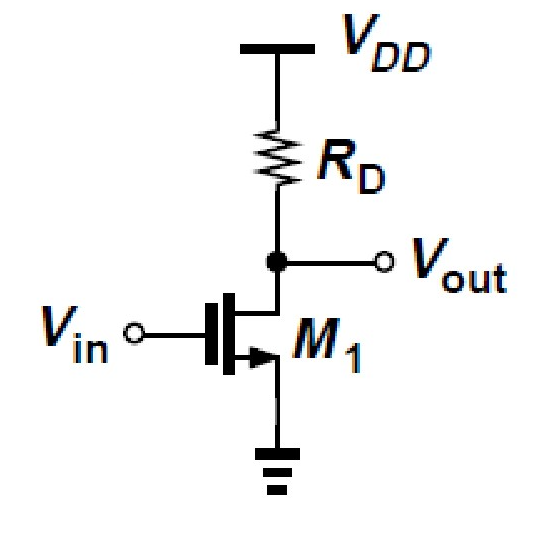
\includegraphics[width=0.8\linewidth]{common-source-R}
    \end{figure}
\end{minipage}
\, 
\begin{minipage}{0.48\linewidth}
    \begin{equation*}
        Gm = -gm_1
    \end{equation*} 
    \begin{equation*}
        R_{out} = r_o||R_D
    \end{equation*}
    \begin{equation*}
        A_v = -gm_1(r_o||R_D)
    \end{equation*}
\end{minipage}\\
* What if $R_D$ is replaced by a DC current source? (slide page 9)\\
* What if $M_1$ is a PMOS?
\end{frame}

\begin{frame}
    \frametitle{Common Source with Diode-Connected Load}
    \begin{minipage}{0.45\linewidth}
        Basic Circuit ($\lambda, \gamma\not= 0$)
        \begin{figure}[H]
            \centering
            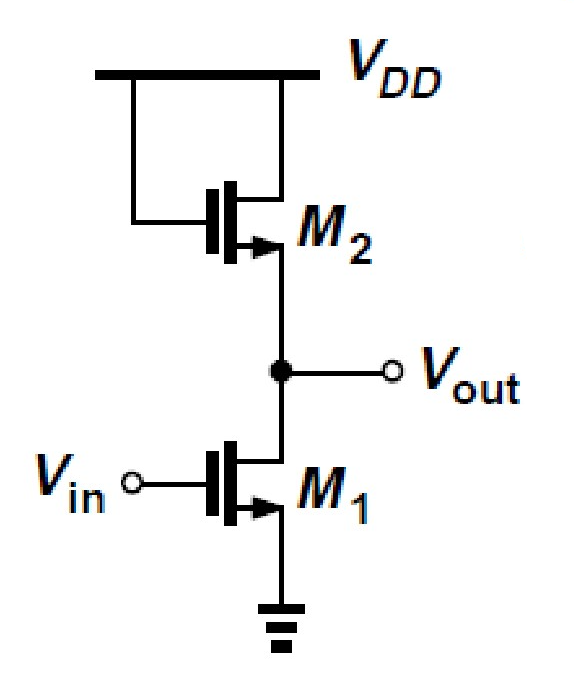
\includegraphics[width=0.8\linewidth]{common-source-D}
        \end{figure}
         
    \end{minipage}
    \begin{minipage}{0.535\linewidth}
        \begin{minipage}{0.3\linewidth}
            \begin{figure}[H]
                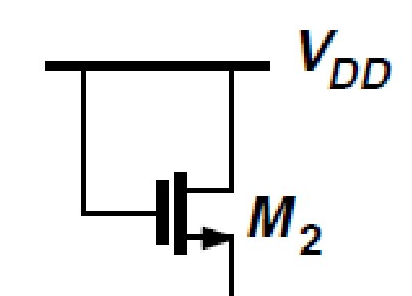
\includegraphics[width=\linewidth]{Rin2}
            \end{figure}
        \end{minipage}
        $\Rightarrow \dfrac{1}{gm_2}||\dfrac{1}{gmb_2}||r_{o2}$\\
        \begin{equation*}
            Gm = -gm_1
        \end{equation*}
        \begin{equation*}
            R_{out} = r_{o1}||\dfrac{1}{gm_2}||\dfrac{1}{gmb_2}||r_{o2}
        \end{equation*}
        \begin{equation*}
            A_v = -gm_1\left( r_{o1}||\dfrac{1}{gm_2}||\dfrac{1}{gmb_2}||r_{o2} \right)
        \end{equation*}
    \end{minipage}
    

\end{frame}
\begin{frame}
    \frametitle{Common Source with Diode-Connected Load (Cont.)}
    \begin{minipage}{0.45\linewidth}
        Basic Circuit ($\lambda, \gamma\not= 0$)
        \begin{figure}[H]
            \centering
            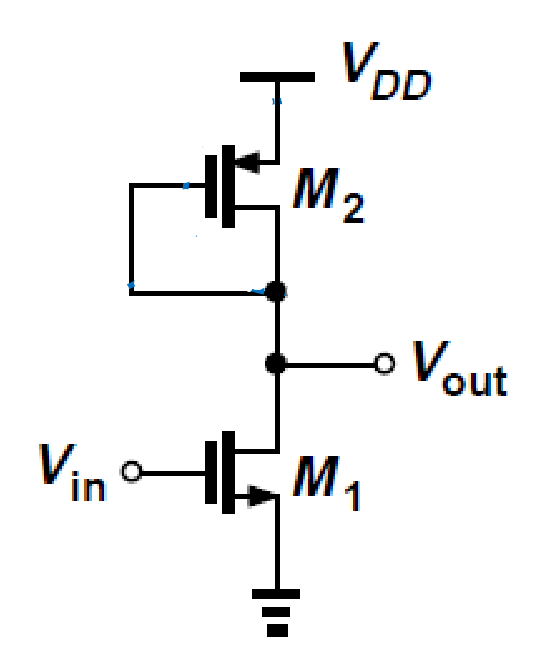
\includegraphics[width=0.8\linewidth]{common-source-D2}
        \end{figure}
         
    \end{minipage}
    \begin{minipage}{0.535\linewidth}
        \begin{minipage}{0.3\linewidth}
            \begin{figure}[H]
                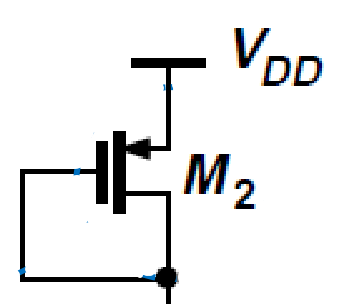
\includegraphics[width=\linewidth]{Rin22}
            \end{figure}
        \end{minipage}
        $\Rightarrow \dfrac{1}{gm_2}||r_{o2}$\\
        \begin{equation*}
            Gm = -gm_1
        \end{equation*}
        \begin{equation*}
            R_{out} = r_{o1}||\dfrac{1}{gm_2}||r_{o2}
        \end{equation*}
        \begin{equation*}
            A_v = -gm_1\left( r_{o1}||\dfrac{1}{gm_2}||r_{o2} \right)
        \end{equation*}
    \end{minipage}
\end{frame}

\begin{frame}
    \frametitle{Common Source with Current-Source Load}
    \begin{minipage}{0.45\linewidth}
        Basic Circuit ($\lambda, \gamma\not= 0$)
        \begin{figure}[H]
            \centering
            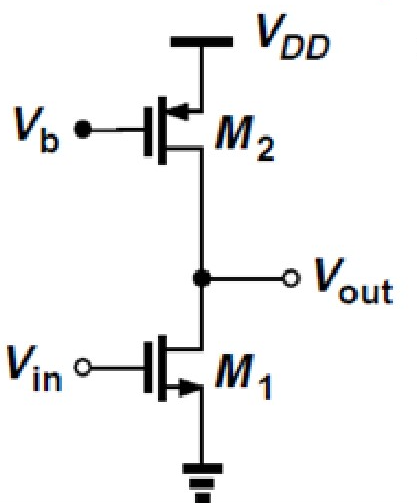
\includegraphics[width=0.8\linewidth]{common-source-C}
        \end{figure}
         
    \end{minipage}
    \begin{minipage}{0.535\linewidth}
        \begin{minipage}{0.5\linewidth}
            \begin{figure}[H]
                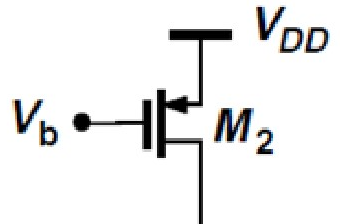
\includegraphics[width=0.8\linewidth]{Rin23}
            \end{figure}
        \end{minipage}
        $\Rightarrow r_{o2}$\\
        \begin{equation*}
            Gm = -gm_1
        \end{equation*}
        \begin{equation*}
            R_{out} = r_{o1}||r_{o2}
        \end{equation*}
        \begin{equation*}
            A_v = -gm_1\left( r_{o1}||r_{o2} \right)
        \end{equation*}
    \end{minipage}
\end{frame}

\subsection{Source Degradation}
\begin{frame}
    \frametitle{Common Source with Source Degradation}
    \begin{minipage}{0.47\linewidth}
        Basic Circuit ($\lambda, \gamma\not=0$)
        \begin{figure}[H]
            \centering
            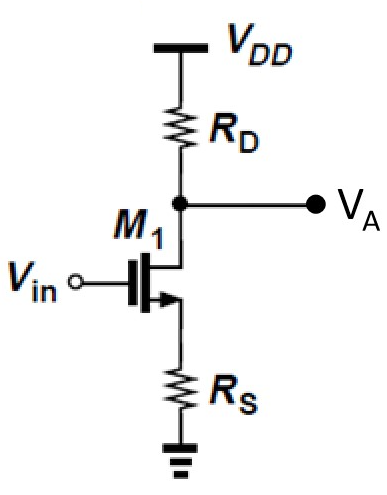
\includegraphics[width=0.8\linewidth]{degradation.png}
        \end{figure}
    \end{minipage}
    \begin{minipage}{0.51\linewidth}
        \begin{equation*}
            Gm = \frac{-gm_{1} r_{o1}}{R_S+r_{o1}+\left(gm_{1}+gmb_{1}\right) r_{o1} R_{S}} 
        \end{equation*} 
        \begin{equation*}
            \begin{aligned}
                R_{out} &= \left[R_{S}+r_{o1}\right.\\
                &\left.+\left(gm_{1}+gmb_{1}\right) r_{o 1}R_{S}\right] || R_{D}
            \end{aligned}
        \end{equation*}
    \end{minipage}\\
    * What if $M_1$ is a PMOS?  
\end{frame}
\begin{frame}
    \frametitle{Common Source with Source Degradation (Cont.)}
    \begin{minipage}{0.45\linewidth}
        Basic Circuit ($\lambda, \gamma\not= 0$)
        \begin{figure}[H]
            \centering
            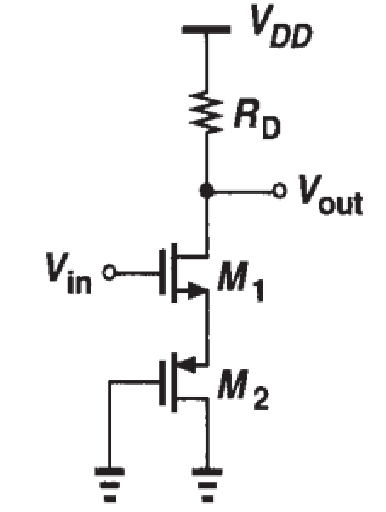
\includegraphics[width=0.8\linewidth]{degradation-D.png}
        \end{figure}
         
    \end{minipage}
    \begin{minipage}{0.5\linewidth}
        \begin{minipage}{0.4\linewidth}
            \begin{figure}[H]
                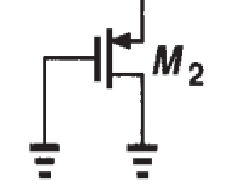
\includegraphics[width=0.9\linewidth]{Rs}
            \end{figure}
        \end{minipage}
        $\Rightarrow \dfrac{1}{gm_2}||\dfrac{1}{gmb_2}||r_{o2}$\\
        \begin{equation*}
            Gm = \frac{-gm_{1} r_{o1}}{R_S+r_{o1}+\left(gm_{1}+gmb_{1}\right) r_{o1} R_{S}} 
        \end{equation*}
        \begin{equation*}
            \begin{aligned}
                R_{out} &= \left[R_S+r_{o1}\right.\\
                &\left.+\left(gm_{1}+gmb_{1}\right) r_{o 1}R_{S}\right] || R_{D}
            \end{aligned}
        \end{equation*}
        \begin{equation*}
            \text{with } R_S \text{ replaced by } \dfrac{1}{gm_2}||\dfrac{1}{gmb_2}||r_{o2}
        \end{equation*}
    \end{minipage}
\end{frame}
%------------------------------------------------
\subsection{Source Follower}
\begin{frame}
    \frametitle{Source Follower}
    \begin{minipage}{0.45\linewidth}
        Basic Circuit ($\lambda, \gamma\not= 0$)
        \begin{figure}[H]
            \centering
            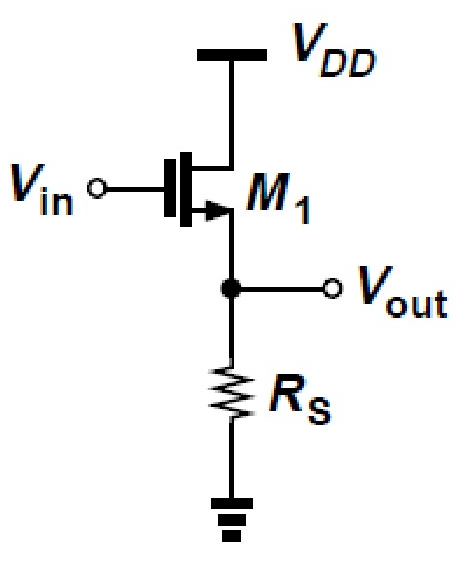
\includegraphics[width=0.8\linewidth]{source-follower-R.png}
        \end{figure}
         
    \end{minipage}
    \begin{minipage}{0.5\linewidth}
        \begin{equation*}
            Gm = gm_1 
        \end{equation*}
        \begin{equation*}
                R_{out} = r_{o1}||R_S||(\frac{1}{gm_1+gmb_1})
        \end{equation*}
    \end{minipage}\\
    * What if $M_1$ is replaced by a PMOS?% TODO: page 36
\end{frame}
\begin{frame}
    \frametitle{Source Follower with Current Source}
    \begin{minipage}{0.45\linewidth}
        Basic Circuit ($\lambda, \gamma\not= 0$)
        \begin{figure}[H]
            \centering
            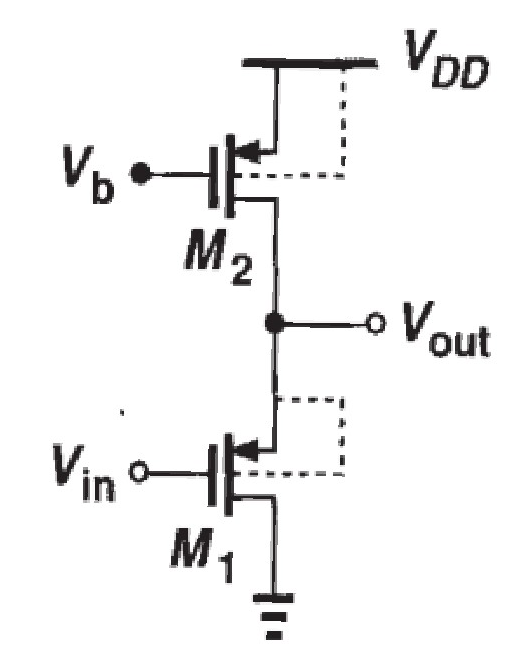
\includegraphics[width=0.8\linewidth]{source-follower-D.png}
        \end{figure}
         
    \end{minipage}
    \begin{minipage}{0.535\linewidth}
        \begin{minipage}{0.5\linewidth}
            \begin{figure}[H]
                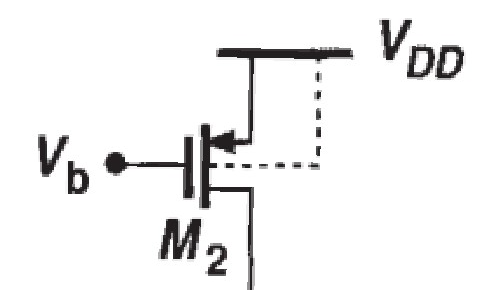
\includegraphics[width=0.8\linewidth]{Rin25}
            \end{figure}
        \end{minipage}
        $\Rightarrow r_{o2}$\\
        \begin{minipage}{0.45\linewidth}
            \begin{figure}[H]
                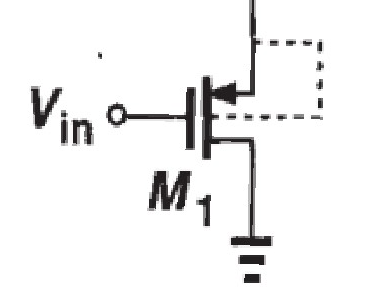
\includegraphics[width=0.8\linewidth]{Rout1}
            \end{figure}
        \end{minipage}
        $\Rightarrow r_{o1}||\dfrac{1}{gm_1}$\\
        \begin{equation*}
            R_{out} = r_o1||\frac{1}{gm_1}||r_{o2}
        \end{equation*}
        \begin{equation*}
            Gm = gm_1
        \end{equation*}
    \end{minipage}
\end{frame}
\subsection{Common Gate}

\begin{frame}
    \frametitle{Common Gate}
    \begin{minipage}{0.4\linewidth}
        Basic Circuit ($\lambda, \gamma\not= 0$)
        \begin{figure}[H]
            \centering
            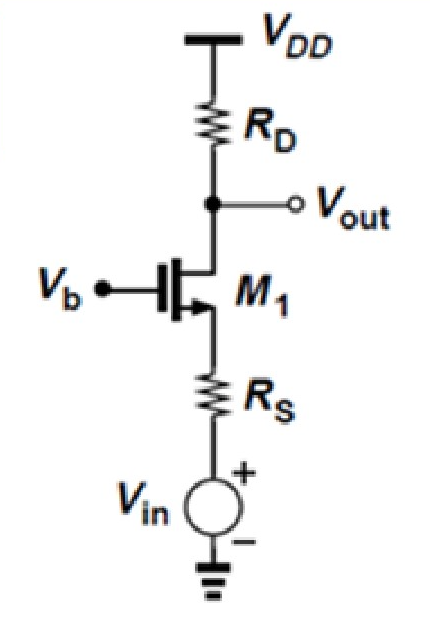
\includegraphics[width=0.8\linewidth]{common-gate.png}
        \end{figure}
    \end{minipage}
    \,
    \begin{minipage}{0.55\linewidth}
        \begin{equation*}
            {G}_{{m}}=\frac{({gm_1}+{gmb_1}) {r}_{{o1}}+1}{{r}_{{o1}}+{R}_{{S}}+({gm_1}+{gmb_1}) {r}_{{o1}} {R}_{{S}}}
        \end{equation*}
        \begin{equation*}
            R_{{out }}=R_{D} \|\left[r_{o1}+R_{S}+(g m_1+g m b_1) r_{o1} R_{S}\right]
        \end{equation*}
        \begin{minipage}{0.26\linewidth}
            \begin{figure}[H]
                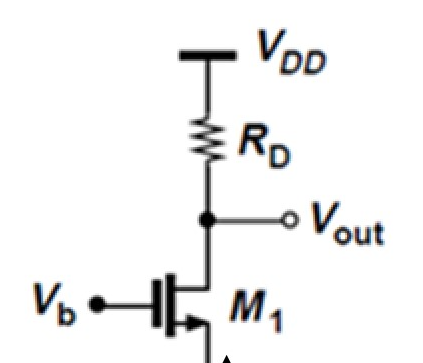
\includegraphics[width=1.1\linewidth]{Rin26}
            \end{figure}
        \end{minipage}
        $\Rightarrow \dfrac{R_{D}+r_{o1}}{1+(gm_1+gmb_1) r_{o1}}$ 
    \end{minipage}\\
    * What if $M_1$ is replaced by PMOS? 
\end{frame}
\begin{frame}
    \frametitle{Complex Common Gate}
    \begin{minipage}{0.4\linewidth}
       ($\lambda, \gamma\not= 0$)
        \begin{figure}[H]
            \centering
            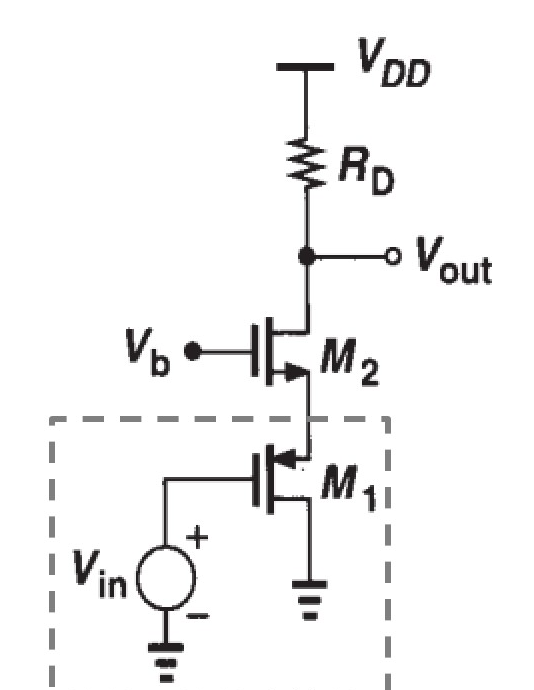
\includegraphics[width=0.8\linewidth]{common-gate2.png}
        \end{figure}
    \end{minipage}
    \,
    \begin{minipage}{0.55\linewidth}
        For
        \begin{minipage}{0.26\linewidth}
            \begin{figure}[H]
                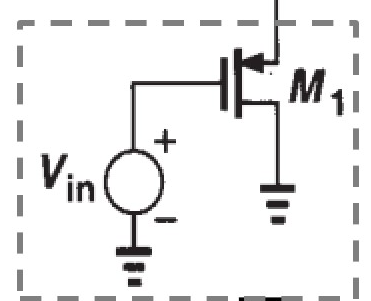
\includegraphics[width=1.1\linewidth]{source-follower2.png}
            \end{figure}
        \end{minipage}
        , take it as a source follower with infinity source resistance. Then we get 
            \begin{figure}[H]
                \centering
                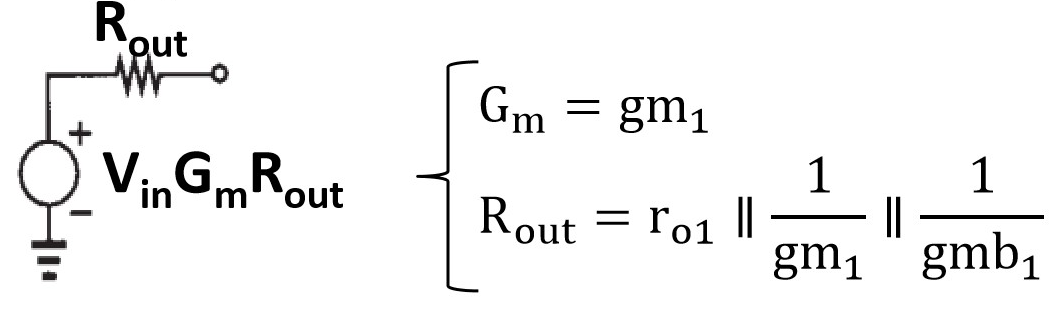
\includegraphics[width=0.9\linewidth]{source-follower3}
            \end{figure}
    \end{minipage}\\
\end{frame}
\begin{frame}
    \frametitle{Complex Common Gate (Cont.)}
    Then
    \begin{minipage}{0.3\linewidth}
        \begin{figure}[H]
            \centering
            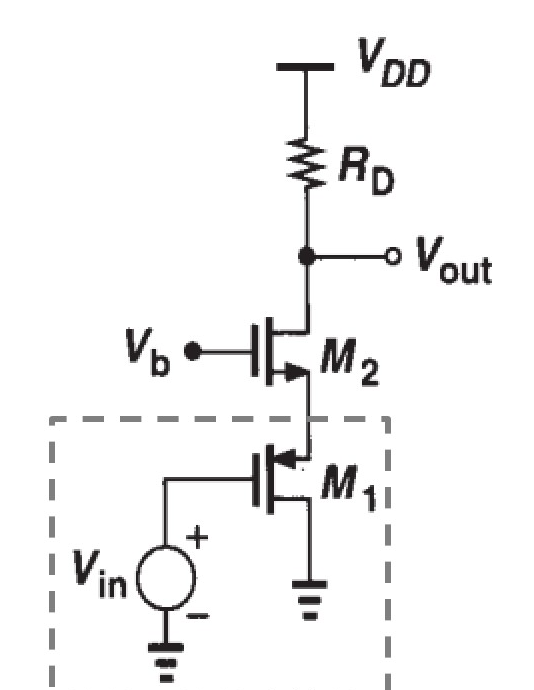
\includegraphics[width=0.8\linewidth]{common-gate2.png}
        \end{figure}
    \end{minipage}
    $\Rightarrow $
    \begin{minipage}{0.3\linewidth}
        \begin{figure}[H]
            \centering
            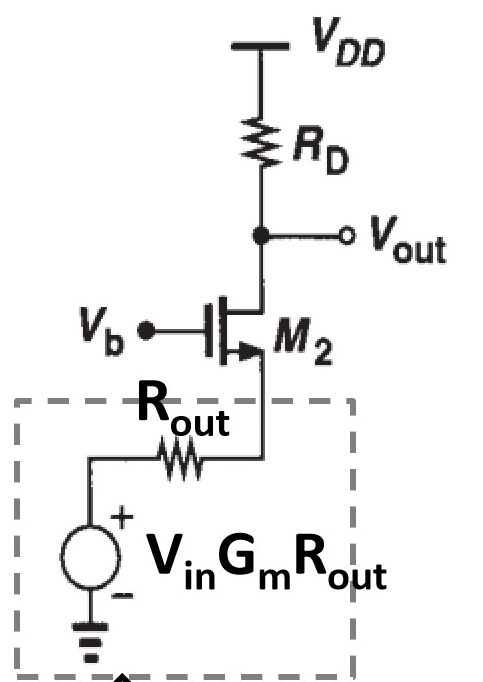
\includegraphics[width=0.7\linewidth]{common-gate3}
        \end{figure}
    \end{minipage}\\
    with 
    \begin{equation*}
        {G}_{{m}}=\frac{({gm_2}+{gmb_2}) {r}_{{o2}}+1}{{r}_{{o2}}+{R}_{{S}}+({gm_2}+{gmb_2}) {r}_{{o2}} {R}_{{S}}}\cdot gm_1\left( r_{o1}||\dfrac{1}{gm_1}||\frac{1}{gmb_1} \right)
    \end{equation*}
    \begin{equation*}
        R_{{out }}=R_{D} \|\left[r_{o2}+R_{S}+(g m_2+g m b_2) r_{o2} R_{S}\right]
    \end{equation*}
    \begin{equation*}
        \text{where } R_S = r_{o1}||\dfrac{1}{gm_1}||\frac{1}{gmb_1}
    \end{equation*} 

\end{frame}

%------------------------------------------------

%------------------------------------------------
%------------------------------------------------

\section{Tips}
\begin{frame}
    \frametitle{Some Tips qwq}
    \begin{itemize}
        \item Understand all the formulas will help.
        \item Please write down partial steps in the exam.
        \item When plotting, please mark your diagram well (peak values, period\dots).
    \end{itemize}
    

\end{frame}
%------------------------------------------------

\begin{frame}
\Huge{\centerline{Good Luck for Your Mid!}}

\end{frame}

%----------------------------------------------------------------------------------------

\end{document} 